\documentclass[11pt,fleqn]{article}

\setlength {\topmargin} {-.15in}
\setlength {\textheight} {8.6in}

\usepackage{amsmath}
\usepackage{amssymb}
\usepackage{color}
\usepackage{tikz}
\usetikzlibrary{automata,positioning,arrows}
\usepackage{diagbox}
\usepackage{stackrel}
\begin{document}
\begin{center}
	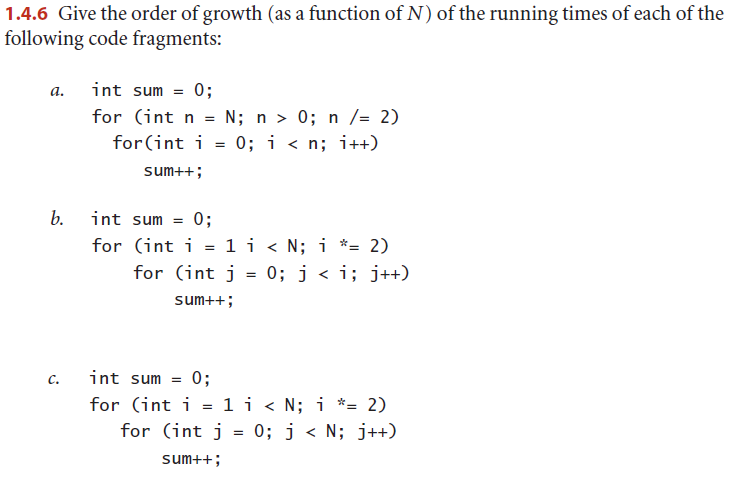
\includegraphics[scale = 1]{1.4.6.png}
	\end{center}
	
Soln

\begin{enumerate}
	\item $O(N)$. For part a, notice how the inner loop dominates because a very large value of N, say $\inf$, the inner loop runtime would be $O(N)$. The outter loop executes that n = N, N/2, N/4, N/8, . . . , 1. By the first case, it is N which is the largest it will ever be, so it is $O(N)$ order of growth.
	
	\item $O(N)$.Note that the times the inner loop is executed are the same as in the previous question
(only in reverse order). So here, the last case would result in $O(N)$ growth.

	\item $NlogN$. Pay close attention to the 2nd loop. It is $j<N$ not $j<i$. This means that for every run, $O(n)$ complexity for inner loop. However, the outter loop is executed $log N$ times since the number of indices seen is halved each time. Therefore, the complexity is $O(nlogn)$
\end{enumerate}


\end{document}

